\documentclass{article}
\usepackage[top=1in,bottom=1in,left=1in,right=1in]{geometry}
\usepackage{amssymb}	% for \mathbb{}
\usepackage{enumerate}	% for \begin{enumerate}[(a)]
\usepackage{mathtools}
\usepackage{bytefield}
\usepackage{rotating}
\usepackage{listings}
\usepackage{subcaption}
\usepackage{caption}
\usepackage{graphicx}
\graphicspath{ {images/} }

\newpage
\title{The MIPS Datapath}
\author{CS61C Spring 2017}
\date{ }
\begin{document}
\maketitle
\tableofcontents
\newpage

\section{The Datapath}
So far we have learned how to translate a C program into MIPS and then into binary, and now we are going to learn how a machine's CPU actually reads that binary and then executes the program in hardware. We call this set of specific hardware in the CPU the MIPS datapath, or the hardware path that an instruction (in binary) takes as it is executed. Figure X displays a diagram of the datapath circuit that we will use throughout this note.

\begin{center}
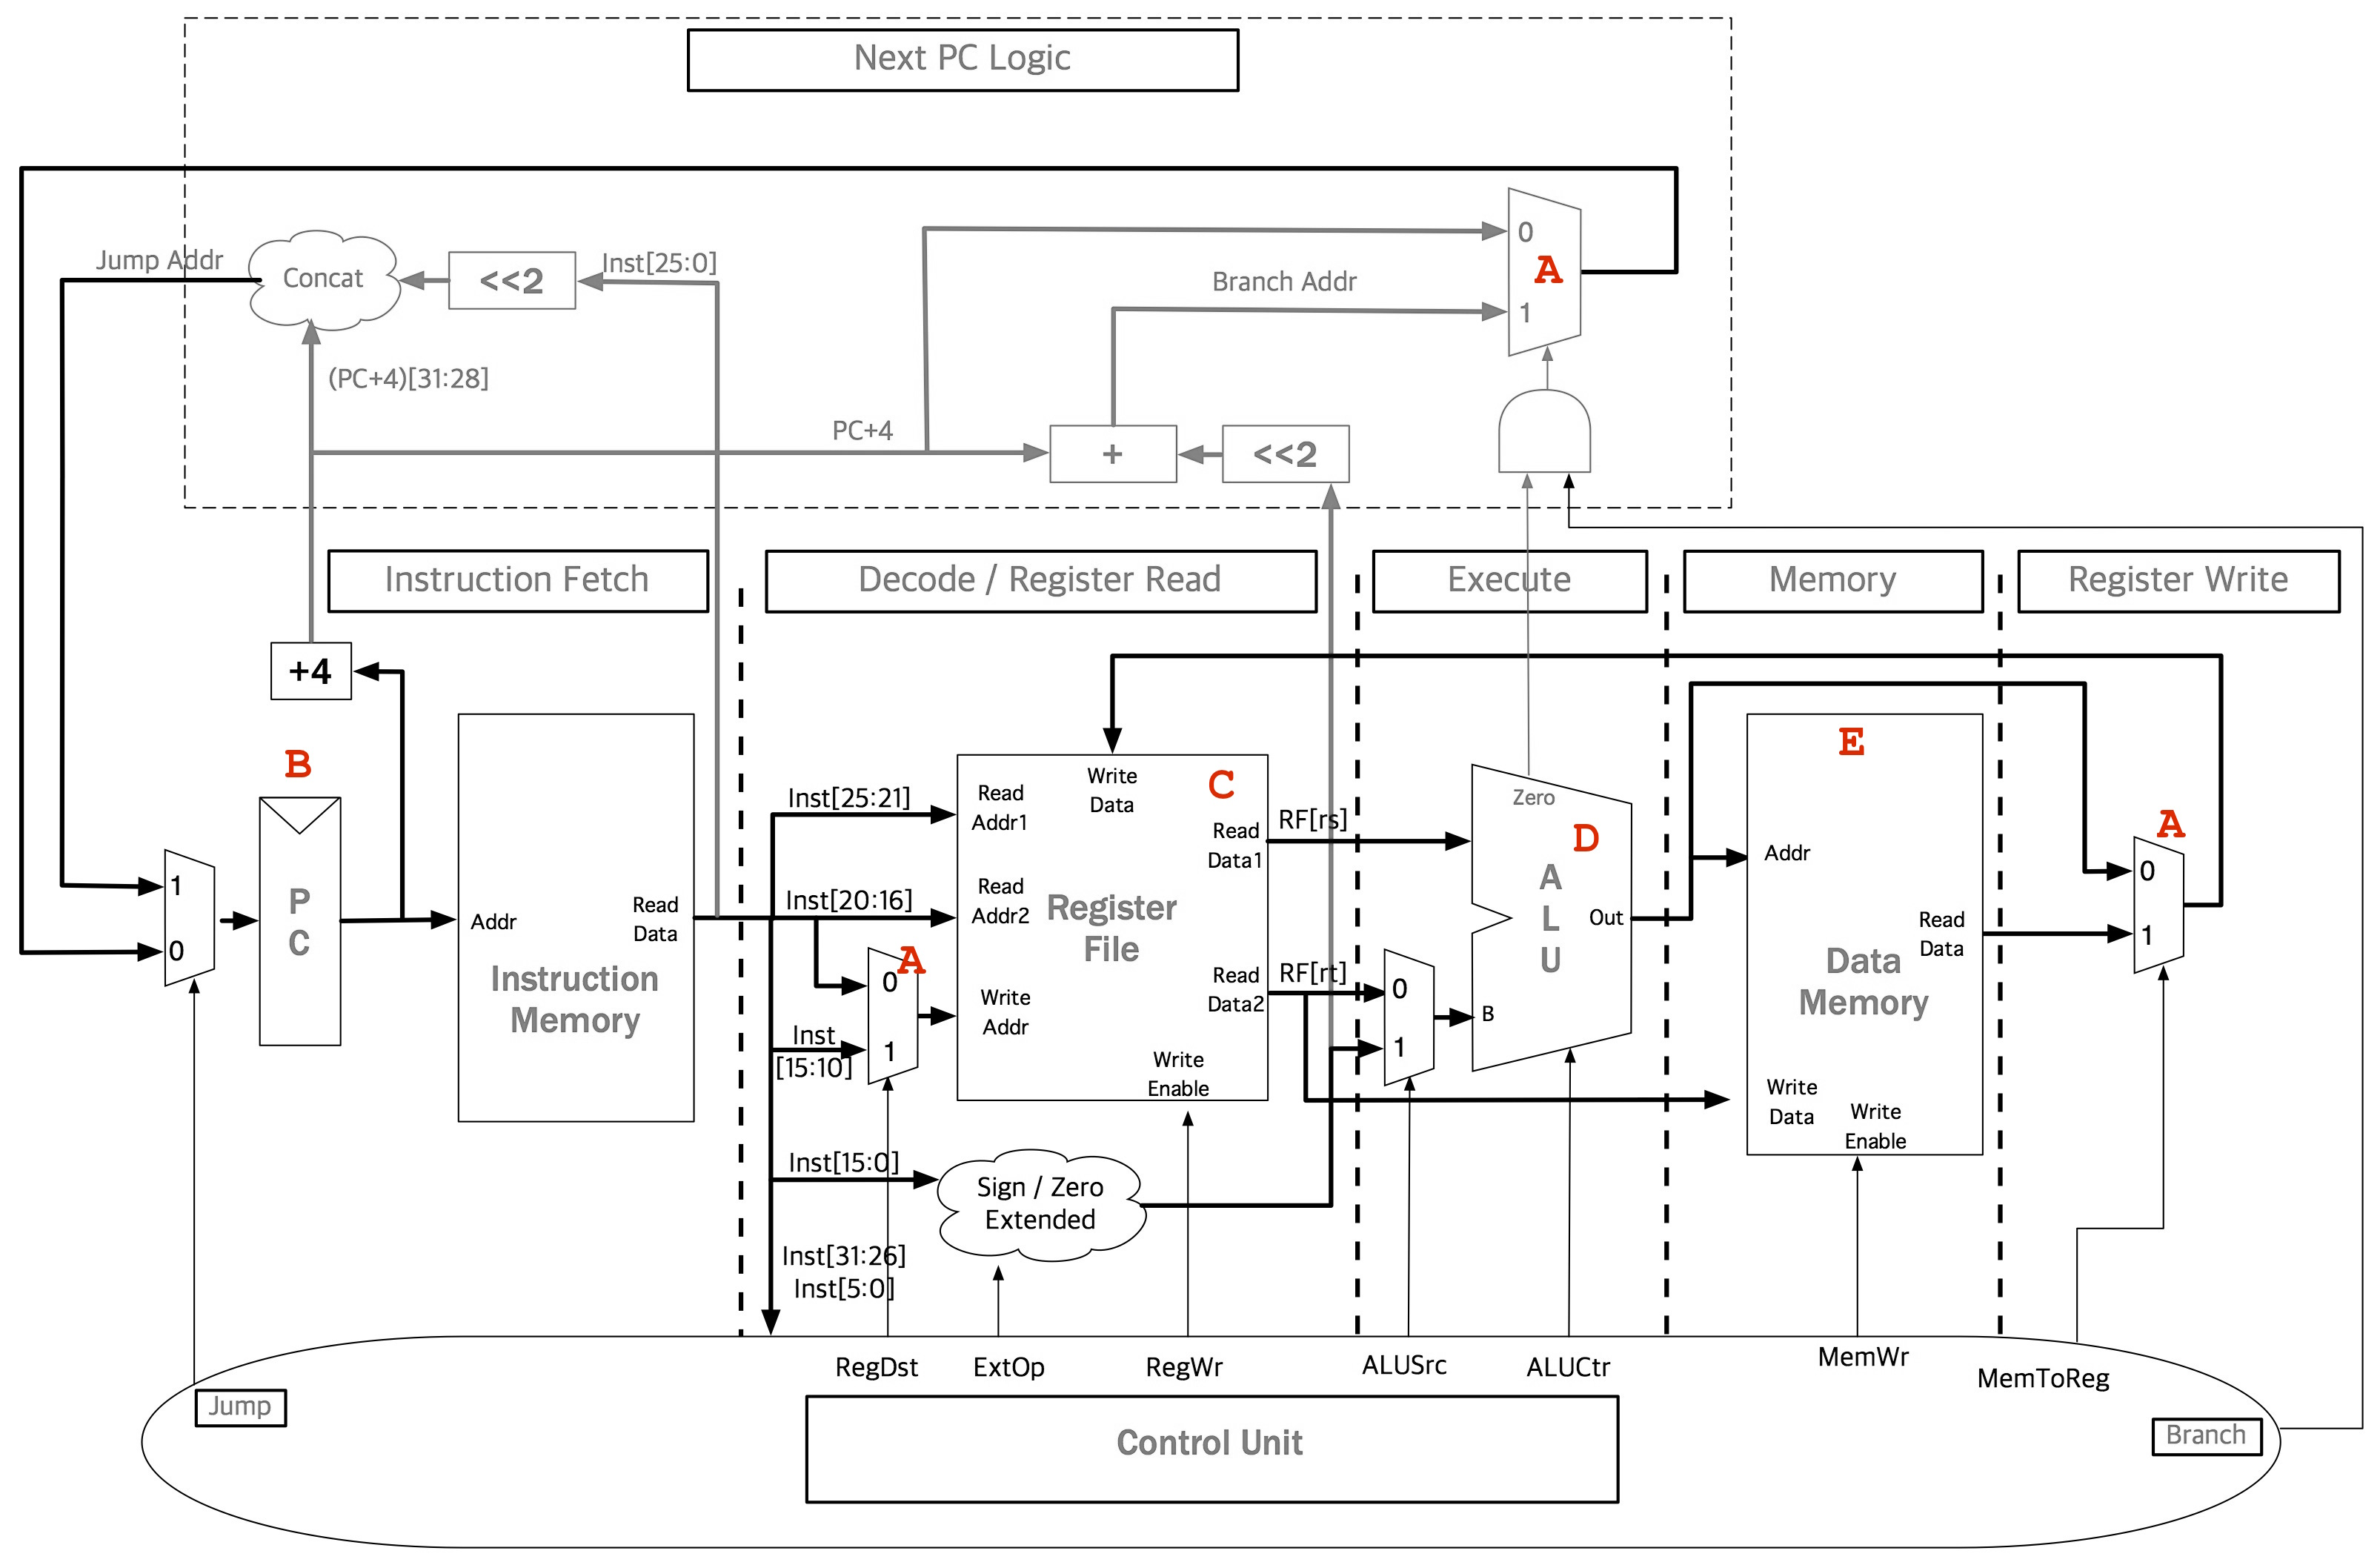
\includegraphics[scale=0.15]{cpu-single-cycle}\newline
\end{center}
\subsection{The Hardware Components}
In order to understand the above diagram, we first explain the key pieces of hardware that are present.

\begin{enumerate}[A)]
\item multiplexes (n-muxes) -- this circuit component takes in $n$ inputs and outputs the input value that is selected by the selector bit(s). The number of selector bits is equal to $log_2(n)$. The multiplexes in the diagram are all 2-muxes, meaning that it will output the topmost input value if the selector bit is 0, and the bottom input if the selector bit is 1.
\item registers -- contain a single 32 bit value that may change at a clock tick
\item RegFile -- this subcircuit is a collection of the 32 registers in the MIPS ISA that also reads and writes to the registers. \textit{Read Register 1} and \textit{Read Register 2} are 5-bit inputs, specifically the register numbers of the registers whose values are to be accessed, and \textit{Read Data 1} and \textit{Read Data 2} are then 32-bit outputs, the values contained in the inputted registers. For example, if the \textit{Read Register 1} input were 2, then the \textit{Read Data 1} output would be the current value of \texttt{\$v0}. If the \textit{Write Enable} control input is 1, then the 32 bit \textit{Write Data} value will be written to the register identified by the 5-bit \textit{Write Addr} input. Otherwise, if \textit{Write Enable} is 0, then the register is not written to.
\item Arithmetic Logic Unit (ALU) -- this subcircuit performs arithmetic operations. It takes in two primary inputs, \textit{A} and \textit{B}, and outputs the result of performing an arithmetic operation on the two inputs. The arithmetic operation is determined by another input, commonly called \textit{ALUCtr}, which is a number that corresponds to the desired operation. The ALU also has other common outputs, such as a binary output of whether or not the two input values are equal.
\item Memory (RAM) -- this is the random access memory that we talked about earlier in this class, and that you're used to. As would be expected, it takes in an address as input and then outputs the value in memory at that address. Like the RegFile, if the \textit{Write Enable} control input is 1, then the value \textit{Write Data} will be written to the memory address identified by the input. Otherwise, if this control input is 0, then no value is written to the given address. \textit{Note:} you may see Memory split into two separate components, Instruction Memory and Data Memory. Both function as described above, but the Instruction Memory is reserved purely for reading instructions (i.e. the code/text segment) from memory and therefore does not have any write inputs, whie the Data Memory can read/write data from the Stack, Heap, and Static segments. 
\end{enumerate}

\subsection{Stages}
The MIPS datapath has five stages that it uses in order to interpret the 32 bits of an instruction and then actually execute the actions of the instruction. Some instructions are active in all five stages, and many are idle in one stage or more. 

\subsubsection{Instruction Fetch (IF)}
In this stage, the next instruction to execute for the program is fetched. The current address in the Program Counter is read, and the instruction (i.e. word of data) at that address is loaded from memory. 

\subsubsection{Instruction Decode (ID)}
In this stage, the 32 bits of the instruction are split into the different fields (depending on the type) that comprise the instruction. The given register numbers for \texttt{\$rs} and \texttt{\$rt} are decoded to the values in the corresponding registers, and the immediate value is extended according to the type of instruction. The register number for \texttt{\$rd} is also inputted into the RegFile (though it may not be used). 

\subsubsection{Execute (EX)}
In this stage, the decoded register value(s) and/or extended immediate from the ID stage are inputted into the ALU, which executes any necessary arithmetic. For arithmetic instructions, the function of the ALU is obvious, while for memory instructions, the ALU will add the immediate/offset to the given address (i.e. the value of \texttt{\$rs}) to calculate the desired memory address. For branch instructions, the ALU will perform \textit{branch comparison}, or comparing if the two register values are equal or not, which means that the CPU will know whether or not to take a branch after the Execute stage. 

\subsubsection{Memory (MEM)}
In this stage, memory is accessed as required by the memory instructions. For load instructions, a value will be read from memory, while for store instructions, a value will be written to memory. Understandably, only memory instructions are then active in this stage.

\subsubsection{Register Write (RW)}
As the name implies, the given register (either \texttt{\$rd} or \texttt{\$rt} depending on the instruction) is written to in this stage.  Therefore, a register's value will not be updated until this stage occurs, and the written register's value can only be trusted as accurate until after this stage.  The PC register is also written to in this stage, either being updated to PC + 4 or to the computed branch/jump address.

\section{Control Signals}
\subsection{What are control signals?}
Notice that the datapath computes many different values (e.g. extended immediate, value of \texttt{\$rt}, etc.), but only some of them are used depending on the instruction. For example, I-type instructions will use the extended immediate as the second input to the ALU, while R-type instructions will use the value of \texttt{\$rt} instead. How does the datapath know which values to use (for example, to feed into the ALU) for a given instruction? Answer: \textbf{control signals}, or control inputs into different hardware components of the datapath that determine the behavior of the individual hardware component. 

Common signals include the selector bits for the different muxes, the \textit{Write Enable} inputs for the RegFile and Memory, and the "which operation" input into the ALU that determines which operation the ALU executes. We use common, more descriptive names for these signals, such as \textit{RegDst} for the signal that determines if \texttt{\$rd} or \texttt{\$rt} should be written to and \textit{MemToReg} for the signal that determines if the value to write to a register is taken from the ALU or from memory. You will be implementing the control signals for the entire MIPS ISA in Project 3, so he rest of the signals are left for you to think about and get familiar with on your own. Note that these names are not standardized and rigidly part of the datapath | the signals necessary for the datapath are dependent on the structure of the datapath and the requirements of the instruction set that it executes. 

\subsection{Determining Control Signal Values}
Since each instruction has its own unique behavior, each instruction also has its own unique set of values for the control signals in the datapath. Some values are shared by groups/types of instructions. For example, all R-Type instructions will have a a \textit{RegWr} value of 1, \textit{RegDst} value of 0, and a \textit{MemToReg} value of 0, since these instructions will always write to a register, write specifically to \texttt{\$rd}, and write the value that results from the ALU. Almost all of the control signal values are binary, but \textit{ALUCtr} is multiple bits since there are more than two ALU operations. Examples of control signal values for some instructions can be found in Figure X. 

A straightforward way of determining the control signal values for an instruction is to walk the datapath from the beginning, and then ask yourself what is the behavior of the instruction as you get to each control signal. For example, let's walk through \textit{addiu}. 
\begin{enumerate}
\item \textit{RegDst}|After fetching the instruction, we enter the ID stage and must decide which register should be written to. Since this is an I-type instruction, \texttt{\$rt} should be written to (i.e. the 0-input of the mux into \textit{Write Addr} of the RegFile). Therefore, \textit{RegDst}should be 0.
\item \textit{ExtOp}|Since \texttt{addiu} has an immediate, we do need to decide how to extend it. As per the Green Sheet, \texttt{addiu} sign extends the immediate, and 1 corresponds to sign extension, so \textit{ExtOp} should be 1.
\item \textit{RegWr}|Does \texttt{addiu} write to a register? It does, so we should enable writing to the RegFile, which means \textit{RegWr} should be 1.
\item \textit{AluSrc}|We now enter the EX stage. Since \texttt{addiu} is an I-type instruction, the inputs into the ALU should be a register value and an immediate (as opposed to two register values). Therefore, the second input into the ALU should be the immediate, which corresponds to the 1-input of the mux into the ALU's second input, and \textit{AluSrc} should be 1.
\item \textit{AluCtr}|Now we must decide which operation to perform on the ALU inputs, and the operation is addition. The mapping of \textit{AluCtr} values to operations is normally provided, and in this case, 2 corresponds to addition|so, \textit{AluCtr} is 2.
\item \textit{MemWr}|Entering the MEM stage, only \texttt{store} instructions write to memory, so \textit{MemWr} should be 0.
\item \textit{MemToReg}|Now in the WB stage, we must decide whether to write a memory value or the result from the ALU back to a register. Since \texttt{addiu} puts the sum of its inputs into the target register, the ALU result (i.e. the 1-input) should be outputted by the corresponding mux. Therefore \textit{MemToReg} should be 1.
\end{enumerate}

\subsection{Deriving Control Signal Values from Instruction Binary}
When the CPU is given the binary of an instruction in order to execute an instruction, it must derive the value of each control signal purely from the binary of the instruction. This is accomplished in two logical parts: 1) Determining the exact instruction 2) Finding the signal values that correspond to that instruction. To determine the exact instruction (e.g. \texttt{addi, lh, beq}), the opcode and the funct are usually AND-ed with some sort of mask to check if the opcode/funct of the given binary matches the opcode/funct for \texttt{addi, lh, beq}, etc. That is, the opcode/funct is checked against the opcode/funct for each possible function, which may seem slow (and would be in an actual circuit if you were to use a comparator to check for equality) but is actually reasonably fast when implemented with logic gates. 

Then to find the signal values, after determining the exact instruction, the resulting values (e.g. "isAdd", "isBeq", etc.) are passed into OR gates. Specifically, instructions are grouped by common control signal values. For example, \textit{AluSrc = 0} for all R-type instructions and \textit{AluSrc = 1} for all I-type instructions, therefore we could write the value of \textit{AluSrc} as a boolean expression: $$AluSrc = isIType = isAddi \lor isAddiu \lor isBeq \lor isBne ... = \lnot isRtype = \lnot(isAdd \land isAddu \land isSub ...)$$ As a circuit, we would then implement this expression as a large OR gate, whose output corresponds to the value of \textit{AluSrc}. A gate would then be constructed for each possible control signal.

\section{Pipelining}

\subsection{The Single Cycle Datapath}
Recall from Synchronous Digital Systems that the clock period for a circuit (such as our datapath circuit) must be long enough for the critical path of the circuit to completely execute|otherwise our registers might end up with intermediate, half-computed values! In the case of the MIPS datapath, the critical path is actually the execution of all five stages. Although most instructions are idle in at least one stage of the datapath, \texttt{load} instructions must go through all five stages in order to execute completely. Therefore, our period needs to be at least the amount of time it takes for all five stages to execute. 

For example, let's say that each stage takes 45 picoseconds for simplicity. Since we want to ensure that every instruction has enough time to execute completely, and some instructions could take as long as five stages to complete, we need to give $5(45 \ ps) = 225ps$ for our clock period. However, if we were able to decrease this clock period, we would be be able to execute more instructions per second...

\subsection{The Pipelined Datapath}
In the single cycle datapath, as an instruction propagates through the stages of the datapath, only one stage is active while the rest are idle. This is inefficient, as each stage will only be used for a fraction of the clock period, even though each stage of the datapath can be active/executing at the same time as the other stages. Pipelining then aims to achieve this parallelism. Logically, the pipelined datapath staggers instructions. This means that as instruction 1 finishes using the Instruction Fetch stage and enters Instruction Decode, instruction 2 enters the Instruction Fetch stage, and as soon as instruction 1 finishes Instruction Decode and enters Execute, instruction 2 finishes Instruction Fetch and enters Instruction Decode, and instruction 3 enters Instruction Fetch, and so on and so forth. This organization is depicted below in a table below. Now, each stage is active in parallel during every clock cycle. 

Hardware wise, the pipelined datapath inserts registers between each stage of the datapath, such that the result of one stage is stored in a register and the following stage then reads from the same register in order to find its input. For example, a register is inserted between the Instruction Fetch and Instruction Decode stages, and it stores the instruction read from memory during the Instruction Fetch stage such that the Instruction Decode stage can decode that instruction during the next clock cycle. Multiple registers may also need to be inserted between stages. For example, between the Instruction Decode and Execute stages, three registers are inserted to store the decoded values of Read Register 1 and Read Register 2, as well as the extended immediate. The presence of these registers ensures that the intermediate value(s) of each stage is safely/accurately stored after each clock cycle, so our clock period no longer needs to be long enough for all five stages to execute but just long enough for one stage (i.e. the longest stage) to finish executing.

The upshot of this pipelining then is a much shorter clock period. In our example, in which each stage is $45ps$, pipelining would reduce our clock period to only $45ps$, a 5x improvement on the single cycle period!

\section{Pipelining Hazards}
Unfortunately, although pipelining decreases our clock period, it introduces new logical hazards that could affect the behavior of the program we are executing on our CPU. There are three main hazards: structural, data, and control. Let's take a look at how pipelining could affect the behavior of the program below:

\begin{center}
\renewcommand{\ttdefault}{pcr}
\begin{lstlisting}[language=C, basicstyle=\ttfamily, keywordstyle=\bfseries, showstringspaces=false, morekeywords={jal, addu, sll, beq, j, sw, addiu, lw, jr, subiu}, numbers=left, stepnumber=1, firstnumber=1, numberfirstline=true]
start:			addiu $t0 $0 4
			subiu $s0 $s0 1
			beq $t0 $t1 branched
not-branched		sw $t0 0($s1)
			sll $t1 $t1 4
branched:		lw $t0 0($s1)
			sw $t1 0($s1)
		...
\end{lstlisting}
\captionof{figure}{A hazardous program.}
\end{center}

\subsection{Structural Hazards}
This hazard arises when a physical piece of hardware, such as memory, cannot be used by two different instructions at the same time. Specifically, since instructions are now staggered as the CPU executes them, it's possible for two stages of the pipeline to both be active and then try to use the same hardware component. For example, Instruction Fetch and Memory may both need to access memory at the same time, but the memory hardware might not support that. Handling this hazard is then usually done in hardware, meaning that these frequently used hardware components are usually wired in order to be able to support simultaneous use. The exact details are generally beyond the scope of this class, so you should just be aware of this type of hazard.

\subsection{Data Hazards}
A data hazard arises when a given instruction relies on a previous instruction updating data, but the given instruction executes before that previous instruction has gotten the chance to update the data. For example, on lines 2 and 3 of our hazardous program, observe that the \texttt{beq} instruction will check if \texttt{\$t0} and \texttt{\$t1} are equal, but the value of \texttt{\$t0} will be first be updated by the preceding \texttt{addiu} instruction. 

Considering the five stages of the datapath then, in order for \texttt{beq} to accurately compare if \texttt{\$t0} and \texttt{\$t1} are equal, we must wait for \texttt{addiu \$t0 \$0 4} to finish its Write Back stage (i.e. updates the value of \texttt{\$t0}) before \texttt{beq \$t0 \$t1 branched} enters its Instruction Decode stage and tries to read the value of \texttt{\$t0}. In a single cycle datapath, we would not have a problem, as the \texttt{addiu} instruction would finish its Write Back stage before the \texttt{beq} even starts its Instruction Fetch stage. However, in our pipelined datapath, observe that the \texttt{beq} enters its Instruction Decode stage when the preceding \texttt{addiu} enters its Execute stage, and well before \texttt{addiu} enters Write Back. Therefore,  \texttt{beq} would compare the old value of  \texttt{\$t0} instead of the updated value!

For the following fixes, consider a hazardous instruction B that depends on a previous instruction A.

 \subsubsection{Stalling}
 The simplest (but possibly not the most efficient) way to handle data hazards is to simply stall the hazardous instruction B so that it does not enter the Instruction Decode stage until after the previous instruction A finishes its Write Back stage. This solves the hazard, but does waste some clock cycles, as some stages will now be idle until instruction A finishes its Write Back stage. Functionally, this involves executing a \textit{NOP} instruction, which has equivalent hex of 0x00000000, and will change no register or memory values (you can decode the NOP instruction and verify this for yourself). % The use of stalling to solve the data hazard in our hazardous program is depicted on the next page.
 
 \subsubsection{Forwarding}
 Even though the value of a register is not updated until the Write Back stage, observe that the new value is actually available by the end of the Execute stage (e.g. for \texttt{addiu \$t0 \$0 4}, the new value, 4, for \texttt{\$t0} will be computed by the end of Execute). Therefore, using a subcircuit called a forwarding unit, we can forward the value computed at the end of the Execute stage of instruction A, to the end of the Instruction Decode/beginning of the Execute stage of instruction B, such that before actually doing any computations with register values, instruction B will receive the updated register values. In the case of our hazardous program, once \texttt{addiu \$t0 \$0 4} finishes computing 4, in its Execute stage, we immediately forward that value to the Execute stage of \texttt{beq \$t0 \$t1 label}, such that the branch instruction will compare the updated value of \texttt{\$t0} (i.e. 4) to the value of \texttt{\$t1}. Effectively, armed with forwarding, we just need to now ensure that the Execute stage of instruction B occurs at least one clock cycle after the Execute stage of instruction A. % The use of stalling to solve the data hazard in our hazardous program is depicted on the next page.
 
 \subsubsection{Write to Register, before Reading from Register}
 There is one detail to note that is common in implementations of the MIPS datapath. Over one clock cycle, registers are written (i.e. udpated) in the first half of the clock cycle, and then read in the second half of the clock cycle. Therefore, if instruction B's Instruction Decode stage occurred in the same clock cycle as instruction A's Write Back stage, then instruction B would read the correct, updated values of registers, as A would first write to the register before B reads the value from that register.
 
 \subsection{Control Hazards}
Normally, in a pipelined datapath, we stagger instructions one after another, meaning that at each clock cycle we start executing the next instruction at PC + 4. However, what if the next instruction is not at PC + 4, but a different address, such as an address we branch or jump to due to a branch/jump instruction? In this case, there is a control hazard, as we should not start executing the instruction at PC + 4, but instead execute the instruction at the Branch/Jump address. Unfortunately, for branch instructions, we will not know whether we take the branch until the branch instruction finishes its Execute stage (unless otherwise specified), so we need some way of delaying the Instruction Fetch stage of the instruction after the branch to occur after the branch instruction's Execute stage. 

More concretely, in terms of our hazardous program, we have a control hazard because our pipelined datapath would start the Instruction Fetch stage of line 4 as soon as line 3 enters the Instruction Decode stage. However, our program may not want to execute line 5 if the branch is taken, but we will not know that information, until line 4 finishes its Execute stage. For the following fixes, please consider a branch instruction B, and then an instruction C that is executed if the branch is not taken and an instruction D that is executed next if the branch is taken.

\subsubsection{Stalling}
Again, we could simply stall our pipelined datapath, such that no instruction starts executing (i.e. starts the Instruction Fetch stage) until instruction B finishes its Execute stage. This will similarly waste clock cycles, but solve our hazard. Notice that we would need to stall for 2 cycles, such that the Instruction Fetch stage of the following instruction (C or D) does not occur until after B's Execute stage.% The use of stalling to solve the control hazard in our hazardous program is depicted on the next page.

\subsubsection{Branch Delay Slot}
Stalling actually is not a bad idea to fix our control hazard, as no matter what, we need to wait until instruction B finishes its execute stage. However, instead of stalling by just executing a dummy NOP instruction, what if we could execute an instruction that we needed to execute anyway? This is the crux of the branch delay slot. Specifically, observe in our hazardous program, that no matter if the branch is or is not taken, line 2 will always happen. Also notice that no other line in our program (before the branch) depends on line 2 (i.e. no other instruction uses \texttt{\$s0}), which means that we could execute it in any order (e.g. before line 1, after the branch instruction, etc.) as long as we make sure it is executed. Therefore, observe that we could switch the order of lines 2 and 3, such that \texttt{beq \$t0 \$t1 branched} is executed before \texttt{subiu \$s0 \$s0 1}, and a stall of one cycle is effectively introduced after the branch instruction. 

\end{document}